%%% Extended English summary of:
%%%   Michael Wessel, "Flexible und konfigurierbare Software-Architekturen
%%%   fuer datenintensive ontologiebasierte Informationssysteme"
%%%   TU Hamburg-Harburg, submitted 2005, defended 14 April 2008.
%%%
%%% Build:  pdflatex english-summary.tex   (twice, for the TOC)
%%%
%%% Typography follows the thesis (URW Bookman, A4) but at 11pt rather than
%%% the thesis's 12pt, which was chosen for the A5 printed edition.

\documentclass[11pt,a4paper,DIV=12,parskip=half]{scrartcl}

\usepackage[T1]{fontenc}
\usepackage[utf8]{inputenc}
\usepackage[english]{babel}
\usepackage{bookman}
\usepackage{microtype}
\usepackage{amsmath}
\usepackage{amssymb}
\usepackage{booktabs}
\usepackage{enumitem}
\usepackage{csquotes}
\usepackage{tikz}
\usetikzlibrary{arrows.meta,positioning}
\usepackage[colorlinks=true,linkcolor=black,urlcolor=black,citecolor=black]{hyperref}

\setkomafont{disposition}{\normalcolor\bfseries}
\addtokomafont{title}{\rmfamily}
\setlist{nosep,leftmargin=*}

% Section headings name thesis chapters, so document-level numbering would
% read "6 Chapter 6: ...". Headings carry the reference themselves.
\setcounter{secnumdepth}{0}
\setcounter{tocdepth}{2}

% Pull-out note, used for calibration remarks and editorial asides
\newenvironment{note}
  {\begin{list}{}{\setlength{\leftmargin}{1.5em}\setlength{\rightmargin}{1.5em}%
                  \setlength{\listparindent}{0pt}}\item[]\small}
  {\end{list}}

% DL notation
\newcommand{\ALC}{\ensuremath{\mathcal{ALC}}}
\newcommand{\Tbox}{\ensuremath{\mathcal{T}}}
\newcommand{\Abox}{\ensuremath{\mathcal{A}}}

\title{Flexible and Configurable Software Architectures for\\
       Data-Intensive Ontology-Based Information Systems}
\subtitle{An extended English summary}
\author{Michael Wessel}
\date{Dissertation submitted 2005, defended 14 April 2008\\
      Technische Universität Hamburg-Harburg\\
      Supervisor: Prof.\ Dr.\ Ralf Möller, Institute for Software Systems (STS)\\
      Logos Verlag Berlin, ISBN 978-3-8325-2162-2\\[0.8ex]
      \small This summary: \today}

\begin{document}
\maketitle

\begin{abstract}
\noindent
This is an extended English summary of a 586-page German dissertation. It
follows the thesis chapter by chapter, at enough depth that a reader can
understand what was built, why, and what the evaluation established, without
reading the German. It closes with a map of which chapters are already
available in English as journal and workshop papers, and which are not.

The thesis asks how to build the software substrate for \emph{ontology-based}
information systems: systems whose behaviour is driven by a formal ontology
rather than a fixed database schema. It answers by designing, implementing and
evaluating a Common Lisp framework across two application domains --- a
deductive geographic information system and Semantic Web retrieval --- and it
argues throughout that such a framework should cover \emph{regions} of the
design space rather than single points.
\end{abstract}

\tableofcontents
\clearpage

\section{How to read this summary}

The thesis divides into three movements. Chapters 1--2 set the problem and the
vocabulary. Chapter 3 derives requirements from two concrete application
domains. Chapters 4--6 build the answer in three layers --- a data model, a
query answering framework, and a reasoner construction kit --- and Chapter 7
evaluates it.

The summary below follows that order. Coverage is proportional to the thesis
except in one place: Chapter 6 is treated more fully than its length alone
would justify, because it is the only chapter never published in any form.

One structural point is worth having in advance, because everything else hangs
from it. The three layers are not independent modules that happen to be
described together. They share a single data model by design, and the thesis's
central engineering argument is that they must: a representation layer, a query
engine and a reasoner that each carry their own internal model will spend their
time translating between models instead of doing work.

\section{Chapter 1: three problems, not one}

Building an ontology-based information system forces three distinct problems at
once, and the thesis argues they cannot usefully be solved in isolation:

\begin{enumerate}
\item \textbf{The representation problem} --- how are the data represented, and
  in what data model?
\item \textbf{The query answering problem} --- how are they retrieved again?
\item \textbf{The inference problem} --- how are the deductions that (2)
  already requires actually carried out?
\end{enumerate}

Conventional information systems avoid all three by fixing a schema and making
the Closed World and Closed Domain Assumptions: absence of data means negative
information, and every relevant object is explicitly modelled. Ontology
languages are more expressive than schema languages, so an ontology-based system
can represent implicit and indefinite information --- and consequently must
admit several possible worlds rather than one. That is where the added value
comes from, and also where the cost comes from: inference becomes necessary to
make implicit domain relationships usable.

\subsection{Regions, not points}

The organising claim is that a framework should cover \textbf{regions of the
design space, not single points}. Committing a framework to one W3C standard
--- the common move at the time, and what JENA did with RDFS and OWL --- fixes
it at a point and forfeits the domains that need something else. The thesis
declines to do this, which is why it ends up defining its own data model rather
than adopting RDF/RDFS.

\subsection{The secondary storage problem}

The central engineering choice is framed through what the thesis calls the
\emph{secondary storage problem}: ontology-based query answering over data too
large for main memory. The obvious approach --- attach a relational or RDF store
through a standard interface --- fails, because when expressive ontology
languages are used the database cannot compute the answers. It can only supply
\emph{candidates}, which must then be loaded into the application layer for
inference. To stay complete, the candidate set must always be a superset of the
true answers; in the worst case that means loading the entire database.

Three architectures are compared.

\begin{center}
\small
\begin{tabular}{@{}llp{5.4cm}@{}}
\toprule
\textbf{Architecture} & \textbf{Inference lives} & \textbf{Cost} \\
\midrule
Layered & outside the store; the DB
        & heavy cross-layer traffic; candidate sets must be supersets;
          DB indexes are \enquote{insufficiently informed} \\[0.4ex]
        & returns candidates & \\[0.4ex]
Semi-integrated & inside the IS core
        & same model discontinuity, better locality \\[0.4ex]
Integrated & database functionality
        & very high implementation effort; no model discontinuity \\[0.4ex]
        & moved \emph{into} the reasoner & \\
\bottomrule
\end{tabular}
\end{center}

Most work of the era took the layered route, reducing ontology expressivity
until the database's own query engine sufficed --- the QuOnto system is cited as
an example, using query rewriting to expand ontology vocabulary down to base
relations, after which SQL suffices. The Instance Store took the dual route,
materialising all derivable facts in advance, at the price of supporting only
unary relations.

This thesis takes the opposite route: integrating database functionality into
the reasoner. It argues that \textbf{high cohesion}, not the usually-sought
loose coupling, is right when two components must share index structures --- and
that the criterion for cohesion is not whether calls are local or remote, but
whether the coupled subsystems share a data model.

\section{Chapter 2: foundations and terminology}

Chapter 2 (29,100 words) exists for two stated reasons: to make the thesis
self-contained, and to fix the author's terminology. It is careful, textbook-grade
exposition, and a reader who knows description logics can skip it --- the thesis
says so explicitly. It is summarised here because the later chapters use its
notation without reintroducing it.

\subsection{Logic}

First-order and propositional logic are introduced to the depth the thesis
needs: syntax, semantics, relational structures, models and the model relation,
satisfiability, validity, entailment and equivalence, the deduction theorem,
compactness, and the undecidability of first-order logic against the
decidability of propositional logic. Herbrand interpretations and Herbrand
models are defined, as are theories, calculi, and soundness and completeness.

Two less standard definitions matter later: \emph{comprehension} and
\emph{constant comprehension}, which give the thesis its way of talking about
first-order formulae as set descriptions --- the bridge it uses to explain both
description logic concepts and query atoms.

\subsection{Knowledge representation}

The chapter then fixes the vocabulary the rest of the thesis leans on: models
and representations; the distinction between data, information and knowledge;
database systems versus information systems versus knowledge-based systems;
rational agents and the architecture of knowledge-based systems;
conceptualizations as sets of formulae; relevant notions from knowledge
organisation, including thesauri; and knowledge representation languages.

The definition of an ontology follows Gruber --- \enquote{an ontology is a
specification of a conceptualization} --- with the stricter variant, a
\emph{shared} conceptualization, noted because sharing is what makes ontologies
useful to multiple agents. Using an ontology means entering an \emph{ontological
commitment}. Only \emph{domain} ontologies are considered; upper ontologies such
as CYC are noted and set aside.

\subsection{Description logics}

The description logic material is the operative part of the chapter. After a
historical sketch, the base logic \ALC{} is defined: concept language, semantics,
semantic properties, and then knowledge bases. A knowledge base is a pair
$\langle \Abox, \Tbox \rangle$. The TBox is a finite set of axioms $C \sqsubseteq
D$ and $C \equiv D$ --- general concept inclusions are allowed --- and the ABox
holds assertions about individuals.

The \textbf{standard inference problems} are then defined along with the
problem reductions between them, and presented as the API of a description logic
system: concept satisfiability, subsumption, ABox consistency, instance
retrieval, and so on. This API framing matters, because Chapters 5 and 6 both
treat these services as things to be implemented, selected and swapped.

More expressive DLs follow: the DL naming scheme, concept-forming operators,
axioms for role properties and complex roles, and \textbf{concrete domains}
with their admissibility condition --- the mechanism by which DLs reach
datatypes and numeric constraints, which becomes important for both guiding
domains. Complexity results are surveyed, and the relationship to modal logics
is drawn via Kripke semantics.

A worked example knowledge base runs through the standard inferences and is
reused later in the thesis. Tableau calculi are introduced as the dominant
approach for deciding satisfiability, with a full \ALC{} tableau calculus given
and its termination, soundness and completeness discussed. Structural
(subsumption) algorithms are covered for contrast. Description logic systems are
then described as engineered artefacts, with RacerPro as the running example.

\subsection{Description logics versus the relational model}

The chapter closes with a comparison the thesis needs repeatedly: the relational
model is characterised, and the differences from DLs are made explicit ---
arity (DLs are essentially unary and binary), the closed versus open world
assumption, unique names, and completeness of answers. From this the notion of
\textbf{ontology-based query answering} is introduced, together with the
value-added services it enables: answers that include entailed facts, queries
formulated in domain vocabulary, and query-level checks such as consistency and
containment.

\section{Chapter 3: two guiding domains, and what they demand}

Chapter 3 derives the requirements. Two domains are analysed in depth; they are
chosen to pull in opposite directions, so that a framework serving both is
demonstrably covering a region rather than a point.

\subsection{Domain 1: a deductive geographic information system}

The first domain uses a real commercial dataset. The \textbf{DISK}
(\emph{Digitale Stadtkarte}) is a digital city map of the Hamburg district of
Öjendorf, sold by the Landesbetrieb Geoinformation und Vermessung Hamburg. It is
cartographically generalised vector data --- less precise than cadastral data ---
whose themes are numeric object keys from the Hamburg object key catalogue:
residential area, public building, arable land, underground station. The thesis
chooses it precisely for that \emph{thematic richness}.

Geo-objects are analysed along three axes: \emph{spatial} aspects, handled
qualitatively through the \textbf{Region Connection Calculus (RCC)};
\emph{structural} aspects; and \emph{thematic} aspects. A DL-inspired
description framework is then laid out in three components --- intensional,
extensional, and query --- and the value-added services of an ontology-based GIS
are identified.

The goal is queries mixing theme and space: \emph{a park containing a pond}, \emph{a
school bordering a main road}. If roles exist for the RCC base relations, such a
concept is directly expressible:
\[
  \mathit{park\_with\_pond} \;\equiv\; \mathit{park} \sqcap \exists
  \mathit{PPI}.\mathit{pond}
\]

This motivates a family of description logics with RCC relations, the
\textbf{$\mathcal{ALC}_{RCC}$ family}. The context is important: the more
general related language $\mathcal{ALCRP}(\mathcal{D})$ had already been shown
\textbf{undecidable}, so the research question is which spatial-thematic
fragments remain decidable.

The domain's conclusion is that three things force \emph{special-purpose}
provers, which standard DL systems cannot supply:

\begin{enumerate}
\item special DLs need special provers (the $\mathcal{ALC}_{RCC}$ family);
\item special inference problems or domain-specific optimisations need them ---
  for instance, closing an RCC ABox over its domain can be done by adding
  unqualified number restrictions, or, better, by a specialised $\exists$-rule,
  which requires an \emph{open} reasoner;
\item the idea of a \emph{spatial ABox}, where individuals are simultaneously
  instances of spatial datatypes in a spatial index, needs provers that are
  aware of that richness.
\end{enumerate}

\begin{note}
\textbf{Still live in 2026.} Two developments postdate the thesis. The
\textbf{$\forall$PO-free fragment} now has a decision procedure, machine-checked
in Lean~4; and the \textbf{decidability of $\mathcal{ALCI}_{RCC5}$ remains
open}, contingent on an unproven width property. This is the one research thread
in the dissertation that is not closed history. See \emph{Where to read more},
below.
\end{note}

\subsection{Domain 2: Semantic Web information retrieval}

The second domain is retrieval over RDF and OWL. The Semantic Web vision and
stack are surveyed --- RDF and RDF Schema, then OWL --- along with the query
languages available at the time. The concrete scenario is the \textbf{Lehigh
University Benchmark (LUBM)}, chosen because its dataset can be generated at
arbitrary size, which makes it the right instrument for a scalability argument.

The analysis of deficits is specific. An expressive query language is needed
that goes beyond what SPARQL and OWL-QL then offered; multi-user operation,
incremental and resource-configurable computation of partial results, and
complete, performant answering of the LUBM queries are all on the list. The
decision is taken to build an \emph{ABox} query language as the basis for the
Semantic Web retrieval language, and the reasoning for that choice is given.

Critically, the OWL reasoner is to be treated as an \textbf{exchangeable
component}. Implementing one is non-trivial, so existing technology (RacerPro)
should be usable bottom-up; but reasoners like RacerPro were built under
different requirements, so special-purpose reasoners may serve better top-down.
Supporting both perspectives means the ABox query language must be not only
\emph{definable} for arbitrary DLs but \emph{realisable} on arbitrary DL systems.

\subsection{The consolidated requirements}

The chapter's summary states three requirements that drive everything after it.

\textbf{A flexible, optionally hybrid, semi-structured graph data model.} It must
represent ABoxes, RDF graphs, RCC networks, the DISK map objects (instances of
spatial datatypes) and the literal data values of an OWL document. It needs a
formal semantics, so that query language semantics can be defined over it;
first-order logic is chosen as the frame. It must support specialised index
structures per instantiation --- spatial indexes for the DISK. Nodes must be able
to carry \emph{rich internal structure}, not merely symbols. And it must give a
uniform abstract view over the differing ABox representations of existing DL
systems.

The thesis addresses the obvious objection directly. Why not RDF/RDFS? Because
rich representations are not readily expressible in it: describing the geometry
of DISK objects through RDF predicates is not sensible --- languages such as
GeoML exist for that --- and it is unclear how an RDF query language would then
exploit a spatial index. It also insists on \emph{node} annotations and not only
edge annotations, since the structure of a richly-structured node is not well
understood as a set of property-value pairs.

\begin{note}
\textbf{This is where the property-graph bridge is.} The requirement is argued
here in exactly the vocabulary of property graphs. The thesis asks for
annotations on \emph{both} nodes and edges; remarks in passing that node
annotations are \enquote{attribute-value or \textbf{property-value pairs}}; and
notes that OWL calls roles \enquote{Properties}. It then rejects the pure
edge-annotation view --- everything decomposed into triples --- as inadequate.

What is worth noticing is that it rejects the property-value-pair view
\emph{as well}: \enquote{the structure of the node itself cannot really be
understood as a set of property-value pairs.} A DISK polygon is an instance of a
spatial datatype with its own index, not a bag of keys and values. The property
graph therefore appears here as a \emph{considered and rejected middle
position}, not as an unwitting anticipation --- and the substrate passes it in
two specific ways:

\begin{itemize}
\item node and edge labels are expressions of an arbitrary description language,
  evaluated by \textbf{entailment} rather than retrieved by lookup --- so an
  edge annotation can be a logical statement a reasoner must prove, not a value
  a store returns;
\item nodes may carry internal structure that no key-value map captures, which
  is what the geometric and spatial substrates need.
\end{itemize}

For a reader arriving from property graphs, GQL, or RDF-star --- all of which
exist because annotating and querying edges as first-class objects turned out to
matter --- this passage, not the formal definition in Chapter 4, is the one to
read. It is the same problem statement, reached in 2005 from the description
logic side, and then pushed past the answer the industry later settled on.
\end{note}

\textbf{A framework for defining query languages}, matching the data model:
optionally hybrid, adaptable per instantiation, formalisable, and efficiently
implementable.

\textbf{Special-purpose provers}, which motivate MiDeLoRa --- designed to work
directly on the same data model, so that a MiDeLoRa ABox is an instance of a
specialisation of it. Sharing representation and index structures between the
query engine and the provers is what avoids model discontinuities and achieves
the cohesion Chapter 1 argued for.

\begin{note}
The thesis is explicit that this framework is motivated by \textbf{pragmatic and
software-engineering reasons rather than theoretical ones}, and argues these
deserve at least as much weight as theoretical aspects in a field it
characterises as primarily theory-driven. That stance is worth noting, because
it explains what the thesis does and does not try to prove.
\end{note}

\section{Chapter 4: the formal framework}

Chapter 4 defines the data model and the query language over it, both formally.

\subsection{The substrate}

A \textbf{substrate} is a node- and edge-labelled graph
\[
  (V,\; E,\; L_V,\; L_E,\; \mathcal{L}_V,\; \mathcal{L}_E)
\]
with $E \subseteq V \times V$, where $L_V : V \rightarrow \mathcal{L}_V$ labels
nodes with expressions of a node description language and $L_E : E \rightarrow
\mathcal{L}_E$ labels edges likewise.

The semantics is first-order. Nodes correspond to constants; a node annotation is
a first-order sentence in prenex normal form whose matrix is in DNF and whose
disjuncts reference that node's constant; edge annotations are ground formulae
in DNF whose disjuncts are binary ground atoms $R(i,j)$. A $\phi$ translation
function makes this explicit, mirroring the standard translation for DLs given
in Chapter 2.

Two further definitions complete the model: the model relation for substrates,
and substrates \emph{with background theory}, where the intensional part of a
knowledge base is supplied separately as a first-order theory. That separation is
the key move --- the substrate is extensional, and the ontology sits beside it.

\subsection{The instantiation zoo}

The flexibility claim is made concrete by instantiating $\mathcal{L}_V$ and
$\mathcal{L}_E$ and defining the resulting semantics each time: propositional
substrates, relational substrates, RCC substrates, geometric substrates with
their model theory, qualitative geometric substrates, and qualitative geometric
RCC substrates. Inference problems for substrates are then posed, and the
substrates needed for the two guiding domains are identified.

\begin{note}
\textbf{A property graph, fused with a reasoner.} The \emph{data substrate} ---
\texttt{data-node} and \texttt{data-edge}, each carrying key--value property
maps, so that properties attach to \emph{edges} and not only nodes --- is in
substance what the industry later called a \textbf{property graph}, implemented
around 2005 and queryable. The author's own SHACL/nRQL analysis is careful about
the claim, and its calibration is the right one to quote: a genuine property
graph, but \textbf{not the first} --- attributed-graph models date to 1984--1994
--- and with \textbf{no documented influence} on Neo4j, Cypher or GQL. That is
\enquote{convergent evolution, not lineage.} What was genuinely singular is the
combination: \textbf{a queryable property graph fused with a tableau DL/OWL
reasoner}, so that query answers include entailed facts rather than only
asserted ones.
\end{note}

\subsection{The generic substrate query language}

Queries are built from three kinds of atom over a set of objects $O_S = V \cup
\mathit{Vars}$, partitioned into individuals and variables:

\begin{itemize}
\item a \textbf{node atom} $(a, v)$ with $a \in O_S$ and $v$ a node query
  predicate from a node query language $\mathcal{L}_{QV}$, where $\Phi(v)[x]$ is
  a first-order formula with one free variable. $\top$ and $\bot$ are required to
  be present;
\item an \textbf{edge atom} $(a, b, w)$ with $w$ from an edge query language
  $\mathcal{L}_{QE}$, where $\Phi(w)[x,y]$ has two free variables;
\item an \textbf{equality atom} $(a, b, =)$, used chiefly as an implementation aid.
\end{itemize}

The semantics of an atom is entailment: a node $i$ matches $(x, C)$ if the
substrate entails $\Phi(C)$ with $x$ bound to $i$. For a propositional substrate
that reduces to propositional deduction; for a DL substrate it is a
theorem-proving request. This is the hinge of the whole design --- \emph{each
query atom is an entailment question, not a lookup} --- and it is what makes the
query engine and the reasoner inseparable. It is also what the implementation's
dispatch mechanism rests on; see \emph{Multimethods}, below.

\textbf{Complex queries} are then defined by an \emph{inductive} grammar. A query
is $\mathit{answer}(\vec{x}) \leftarrow k$, and a body $k$ is either an atom or
one of four constructs over bodies $k_1, \ldots, k_n$:

\begin{center}
\small
\begin{tabular}{@{}ll@{}}
\toprule
$\setminus (k_i)$ & negation as failure \\
$(k_1 \wedge \cdots \wedge k_n)$ & conjunction \\
$(k_1 \vee \cdots \vee k_n)$ & disjunction \\
$\pi(\vec{x})\, k_1$ & projection, where every object of $\vec{x}$ occurs in $k_1$ \\
\bottomrule
\end{tabular}
\end{center}

Because the grammar is inductive, the operators apply to \emph{arbitrary
sub-bodies} rather than only to atoms. That is the substantive point: $\pi$ is a
compositional projection operator producing a new relation from a sub-body --- a
subquery --- and $\setminus$ applies to a body, so $\setminus(\pi(\vec{x})\,k)$
is a \emph{negated projected subquery}. The remaining machinery follows:
$\mathit{objects}(k)$ and $\mathit{vars}(k)$, the extension of $\Phi$ to bodies,
the semantics of a query, and a $\models_{NAF}$ relation.

\begin{note}
\textbf{Two negations, deliberately kept apart.} The thesis is careful that
negation-as-failure is \emph{not} the negation already available inside an atom.
Even when the node query language offers it --- $(a, \neg C)$ in an
$\mathcal{ALC}$ instance query --- the complement $V \setminus (a,C)^\mathcal{E}$
and the extension $(a, \neg C)^\mathcal{E}$ do not coincide, because substrates
make no closed-world assumption. One is \emph{not provably $C$}; the other is
\emph{provably not $C$}. A query language over an open-world knowledge base needs
both, and needs the boundary between them visible rather than conflated. Few
query languages of the period drew it explicitly.
\end{note}

\begin{note}
\textbf{What SPARQL and SHACL reached later.} Subqueries, negated subqueries,
projection operators and the mixing of the two negations were all present in this
grammar in 2005 and implemented in nRQL. SPARQL~1.0 became a Recommendation in
January 2008 with neither subqueries nor negation; both arrived with
SPARQL~1.1 in March 2013, as \texttt{NOT EXISTS}, \texttt{MINUS} and nested
\texttt{SELECT}. SHACL's constraint patterns cover much of the same ground again
--- a coding of the W3C SHACL Core test suite finds 73.5\,\% of its constraints
have a direct nRQL counterpart.

The distinctive part is not that the individual features appeared early. It is
that they were defined over \emph{one inductive grammar}, so they compose: any
body can be projected, and any projection can be negated. Feature lists converge;
a grammar that makes them compose is a design.
\end{note}

Considerable work then goes into \textbf{semantics-preserving transformations}:
negation normal form, disjunctive normal form, the clause set $\mathcal{M}(q)$,
arity unification across disjuncts, and individual substitution. These are what
make the optimiser of Chapter 5 possible.

Three further readings of the same language are given: a first-order
interpretation, a logic-programming perspective, and an \textbf{alternative
algebraic semantics} built from projection, cylindrification, diagonals and the
$\mathbf{1}$-vector --- essentially a cylindric-algebra account, which connects
the language to relational algebra.

\subsection{Inference problems for queries, and the QBox}

Queries themselves become objects of inference: query satisfiability,
unsatisfiable and tautological queries, and \textbf{query subsumption} and
equivalence. From these comes the \textbf{QBox} --- a directed acyclic graph
whose nodes are queries and whose edges record immediate subsumption, always
containing a $\top$ and a $\bot$ query.

The QBox is the query-level analogue of a TBox taxonomy, and it pays for itself
twice: the stored results of \emph{subsuming} queries serve as superset caches
for candidate generators, and the stored results of \emph{subsumed} queries can
be returned immediately as subsets of the answer. Computing it requires a
decision procedure for query subsumption, which Chapter 5 supplies for two of the
four languages.

Finally \textbf{hybrid queries} are defined, spanning several substrates at once,
with a notion of $*$-consistent variable binding to tie the bindings together.

\section{Chapter 5: the software realization}

Chapter 5 (46,500 words) is the longest, and turns the formal model into Common
Lisp. It divides into the data model realization, the query engine, and four
concrete query languages.

\subsection{Realizing the substrate}

The object-oriented design starts from base classes and methods, then addresses
three concerns. \textbf{Transient, persistent and virtual substrates} are
handled through multiple inheritance, so persistence is a mixin rather than a
separate hierarchy. \textbf{Physical representation independence} is achieved
through iterators: provers and the query engine touch nodes and edges only
through iterators and accessors, never through a concrete representation. And a
family of \textbf{standard substrate classes} is supplied --- the simple
substrate, the data substrate, the disjunctive edge substrate, the RBox
substrate, the JEPD substrate, the RCC substrates, description logic substrates,
hybrid substrates and the geometric substrate --- alongside standard description
classes. Substrates for both guiding domains are then instantiated: the map
substrates for the GIS, and RacerPro-backed substrates for Semantic Web
retrieval.

\subsection{Multimethods: choosing the reasoner per atom}

One thread runs through the whole architecture and is easy to miss, because it
lives in the programming language rather than the formalism. Chapter 4 defines
the meaning of a query atom as \emph{entailment}. Chapter 5 implements that
entailment as a \textbf{binary generic function}, dispatched on the pair
\emph{(description or node type, query atom type)} --- which single-dispatch
object systems cannot express directly, and which CLOS gives for free.

In the sources, \texttt{matches-p} is specialised on exactly those pairs:

\begin{center}
\small
\begin{tabular}{@{}ll@{}}
\toprule
\textbf{Query atom class} & \textbf{Description / node class} \\
\midrule
\texttt{substrate-simple-node-query}    & \texttt{simple-node-description} \\
\texttt{substrate-racer-node-query}     & \texttt{racer-node-description} \\
\texttt{substrate-predicate-node-query} & \texttt{substrate-node} \\
\multicolumn{2}{@{}l@{}}{\itshape …and the corresponding edge variants} \\
\bottomrule
\end{tabular}
\end{center}

Each delegates to \texttt{implies-p}, itself generic: its default method is a
syntactic CNF implication test for data substrates, while a DL-backed description
resolves instead to description logic entailment. Retrieval is selected the same
way --- \texttt{retrieve-\allowbreak matching-\allowbreak objects} carries a generic method on
\emph{(substrate, unary query)} and a specialised one on \emph{(racer substrate,
unary query)}. Query subsumption uses a third such multimethod,
\texttt{entails-p}, defined on \emph{query $\times$ query}.

Multiple inheritance then makes the class space a \emph{product lattice} rather
than a tree. Classes are formed by crossing a substrate family with a role:

\begin{center}
\footnotesize
\begin{tabular}{@{}l@{\;=\;}l@{}}
\toprule
\texttt{data-substrate-node-query} & \texttt{data-substrate-query} $\times$ \texttt{unary-query} \\
\texttt{data-substrate-edge-query} & \texttt{data-substrate-query} $\times$ \texttt{binary-query} \\
\texttt{midelora-instance-retrieval-query} & \texttt{midelora-abox-query} $\times$ \texttt{instance-retrieval-query} \\
\texttt{mirror-sql-data-substrate} & \texttt{sql-data-substrate} $\times$ \texttt{mirror-data-substrate} \\
\bottomrule
\end{tabular}
\end{center}

The consequence is the point. \textbf{Which entailment procedure runs is decided
per atom, at runtime, by method resolution}, and behaviour can be defined at
whichever level of the lattice fits --- generically for all substrates, or
specifically for one combination. A propositional substrate gets propositional
deduction; a DL substrate a tableau prover; an RCC substrate composition-table
reasoning; a geometric substrate a spatial index. Same query language, same atom
syntax, different entailment relation, chosen by the pair.

\begin{note}
\textbf{Entailment regimes, reached from the other side.} SPARQL arrived at a
comparable idea with \emph{entailment regimes} --- one query syntax, several
entailment relations (RDF, RDFS, D-entailment, OWL 2 Direct and RDF-Based
Semantics, RIF), so that basic graph pattern matching can be interpreted under a
chosen semantics. That became a W3C Recommendation in March 2013, with the
underlying work circulating in the working group for some years before.

The mechanism here differs in grain. A SPARQL entailment regime is fixed
\emph{per query or dataset}: one regime governs the whole evaluation. Here the
method is selected \emph{per atom, against the substrate that atom touches}, so a
single hybrid query can have its concept atoms answered by a DL reasoner, its
spatial atoms by a geometric index and its data atoms by a syntactic test --- in
one conjunction, under one semantics.

This is also the mechanism behind the thesis's central claim. Covering
\emph{regions of the design space rather than points} is not a slogan about
generality: the dispatch lattice \emph{is} the region, and a new point in it is a
new class plus the methods that distinguish it. The same construction reappears
one layer down as the MiDeLoRa space --- a prover chosen by \emph{task $\times$
logic $\times$ ABox class} --- applied to reasoners instead of atoms.
\end{note}

\subsection{The query answering engine}

Query processing is a seven-stage pipeline.

\begin{center}
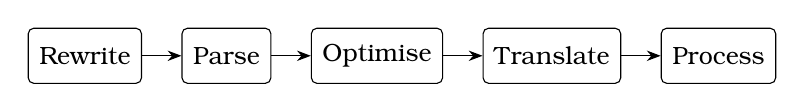
\begin{tikzpicture}[
   node distance=5mm,
   box/.style={draw, rounded corners=2pt, minimum height=7mm, inner xsep=4pt,
               font=\small},
   >={Stealth[length=5pt]}]
  \node[box] (a) {Rewrite};
  \node[box, right=of a] (b) {Parse};
  \node[box, right=of b] (c) {Optimise};
  \node[box, right=of c] (d) {Translate};
  \node[box, right=of d] (e) {Process};
  \draw[->] (a) -- (b); \draw[->] (b) -- (c);
  \draw[->] (c) -- (d); \draw[->] (d) -- (e);
\end{tikzpicture}
\end{center}

Optimisation (stage 4) operates on queries in normal form and has three parts:
\emph{semantic} optimisation, \emph{determination of existential variables} ---
variables whose bindings need not be enumerated, only shown to exist --- and
\emph{heuristic syntactic} optimisation.

\paragraph{The heuristic optimiser.}
This is the part that matters most, and it is a genuine query optimiser of the
kind databases have, applied to DL ABox queries. Different variable binding
orders for a disjunction-free, projection-free query give very differently
performing \textbf{query execution plans}. A plan is the processing order of the
conjuncts, written as a vector $\langle a_1, \ldots, a_n \rangle$; a query with
three conjuncts admits $3! = 6$ plans.

An atom's position in the plan determines its \textbf{role}. A unary atom is
either a \emph{candidate generator} or a \emph{tester} (filter). A binary atom
takes one of four roles depending on how many of its objects are already bound:
generator, \emph{successor generator}, \emph{predecessor generator}, or tester.

The consequence is concrete. For $(x,C) \wedge (y,D) \wedge (x,y,R)$, the plan
$\langle (x,C), (x,y,R), (y,D) \rangle$ makes $(x,C)$ a generator, $(x,y,R)$ a
successor generator and $(y,D)$ a tester. The plan $\langle (x,C), (y,D),
(x,y,R) \rangle$ instead makes both $(x,C)$ and $(y,D)$ generators, forcing a
cross product of size $|(x,C)^{\mathcal{E}}| \times |(y,D)^{\mathcal{E}}|$ with
$(x,y,R)$ reduced to a filter. Every variable needs a generator; the optimiser's
job is to choose among the candidates by cost estimate.

\paragraph{Translation and processing.}
Stages 5--7 determine the query processing functions and generate them from
\textbf{code templates} at compile time, so the cost of late binding is resolved
once rather than per call. Function calls within those processing functions are
minimised. Answer generators are \emph{incremental and stream-based}, and
\emph{informed} --- they consult index structures rather than enumerate blindly.
The need for $n$-ary generators and testers is addressed, as is the use of index
structures generally, support for hybrid substrate query languages, the query
lifecycle and API, the concrete syntax, and the library of standard atoms
(simple atoms, RacerPro description atoms, and $\lambda$-atoms).

\subsection{The optimisations, and what each was worth}

The thesis treats query optimisation as a first-class subject and --- unusually
--- measures each technique separately, reporting the ones that disappointed as
plainly as the ones that worked. The full set:

\textbf{Semantic optimisation} rewrites the query graph before planning, by two
means. \emph{Query classification} inserts the query into the QBox, so a
subsuming query's stored answers can serve as a superset cache for candidate
generation and a subsumed query's answers can be returned outright; a query
found equivalent to $\top$ is flagged as tautological and one equivalent to
$\bot$ as unsatisfiable, short-circuiting the evaluation entirely.
\emph{Query realization} --- which the thesis states had not previously been
investigated --- is the query analogue of ABox realization: a conjunctive query
is augmented with \emph{implied atoms} so the search is better informed. Given
$(x,\forall R.D) \wedge (x,C) \wedge (x,y,R)$, any $y$ must be a $D$ instance,
but no atom says so, and a generator for $y$ would enumerate $\top$ instances
instead of $D$ instances. Adding the implied $(y,D)$ and $(y,\exists R^{-1}.C)$
cuts the branching factor. The thesis frames this explicitly in constraint-solving
terms --- it is \emph{forward checking}, and what it avoids is \emph{thrashing}
--- and is candid about the trade-off: more specific implied atoms make candidate
generation itself more expensive, so the suggested criterion is to add only atoms
an index can support.

\textbf{Existential variables.} A variable that appears in no other atom and not
in the head need only be \emph{witnessed}, not enumerated; generators stop after
the first binding.

\textbf{Heuristic plan optimisation.} The conjunct ordering, as described above:
each atom takes a role (generator, successor generator, predecessor generator,
tester) determined by its position, and the optimiser costs the alternatives.

\textbf{Code-template translation.} Processing functions are generated by nesting
code templates at compile time, so the whole query collapses into a single
function for the root of the query graph --- eliminating both the per-node
\texttt{funcall} chain and graph traversal at answering time.

\textbf{Informed, incremental generators}, which consult index structures and
stream results, plus efficient processing functions for role atoms, and $n$-ary
generators and testers.

\begin{center}
\small
\begin{tabular}{@{}lll@{}}
\toprule
\textbf{Technique} & \textbf{Measured} & \textbf{Verdict in the thesis} \\
\midrule
Heuristic plan optimisation & up to $10{,}000\times$ & indispensable \\
Existential variables & $1.013\times$ typical & negligible in practice… \\
 & $350\times$ worst case & …but decisive on cross-product queries \\
Query classification (QBox) & $2.1\times$ & effective, and grows with query count \\
Code-template translation & $1.568\times$ & \enquote{not as effective as hoped} \\
Query realization & --- & novel; not evaluated in time \\
\bottomrule
\end{tabular}
\end{center}

Two of these deserve comment. The heuristic optimiser is not an optimisation but
a precondition: without it, even simple queries over a single university
department do not finish in acceptable time. And the QBox figure understates the
mechanism, because it is measured over only four queries. The underlying numbers
are striking --- a DISKQL query over 2,694 map objects takes \textbf{155\,s}
cold; a more specific query that finds it as a parent then takes \textbf{17\,s},
the next \textbf{0.38\,s}, and a fourth, classified between two existing nodes,
\textbf{0.72\,s}. Without classification the same four cost 161, 123, 45 and 41
seconds. The saving compounds as the QBox fills.

\begin{note}
\textbf{On priority.} These techniques were documented and implemented in
2004--05, and several were evaluated. Individual ingredients have longer
lineages --- subsumption-based caching goes back to work the thesis itself cites
from 1994, forward checking to constraint solving, generator/tester plan
ordering to relational query optimisation. What is specific here is the
\emph{combination}: this set of techniques assembled for conjunctive query
answering over description logic ABoxes, implemented in a system with users, and
measured technique by technique. That is a claim that rests on the dates and the
numbers above, both of which are checkable.
\end{note}

\subsection{Four query languages on one framework}

\begin{center}
\small
\begin{tabular}{@{}lll@{}}
\toprule
\textbf{Language} & \textbf{Substrate} & \textbf{Purpose} \\
\midrule
DSA    & data substrate        & queries over plain data values \\
BAA    & ABox                  & generic conjunctive ABox query language \\
nRQL   & ABox + data substrate & the Semantic Web / OWL retrieval language \\
DISKQL & spatial map substrate & spatial-thematic queries over the DISK \\
\bottomrule
\end{tabular}
\end{center}

The \textbf{BAA} is the generic ABox query language. Its treatment includes
efficient processing functions for role atoms, an algorithm for deciding
\textbf{query subsumption}, and an algorithm for deciding query
\textbf{satisfiability}, each worked through an example.

\textbf{nRQL} is the one that reached users, and it gets the most space. Refined
requirements are derived first: concrete domain support, OWL-specific support,
and modes for incomplete and two-phase processing. Its substrate is designed in
two parts --- an ABox substrate and a data substrate --- and then the language
itself: query concepts, \textbf{constraint atoms}, \textbf{head projection
operators} for retrieving concrete-domain individuals and told values, and
hybrid queries. Concrete syntax and worked examples follow, including the LUBM
queries written in nRQL.

The operational design is where nRQL differs most from its contemporaries.

\begin{itemize}
\item \textbf{Four modes, 0--3}, of increasing completeness, with mode 3
  complete. The incomplete modes work by enriching nRQL's local cache and index
  structures with additional entries derivable by \enquote{simple} inference ---
  described as fixpoint iterations that maximise told information. Crucially,
  \emph{the original ABox is never modified}; the enrichment exists only in the
  caches. Mode 0 uses told information alone, splitting conjunctive concept
  assertions so that $i : C_1 \sqcap \cdots \sqcap C_n$ yields each $i : C_i$.
  The incomplete modes reach acceptable completeness only for concept atoms
  whose query concept is \emph{atomic}, since the enrichment processes cannot add
  arbitrary concept assertions.
\item \textbf{Two-phase modes}, which return a cheap partial answer first and
  refine it, and \textbf{incremental} and concurrent answering.
\end{itemize}

Implementation covers the cache and index structures, the parser, the query
syntax graph classes and the processing functions, heuristic refinement of the
optimiser's cost estimates, the RacerPro support needed for two-phase operation,
and a prototypical Semantic Web retrieval scenario with an OWL tree browser.

\textbf{DISKQL} and the \textbf{DLMAPS} system close the chapter: use of the map
substrates, refined requirements, spatial node atoms and spatial edge atoms, the
concrete syntax demonstrated on the DISK reference queries, and an algorithm for
deciding subsumption between restricted DISKQL queries. The implementation
covers the end-user syntax, the spatial atoms, adapted cost estimates for spatial
edge atoms, and a \emph{Query Inspector} GUI.

\section{Chapter 6: MiDeLoRa --- the unpublished chapter}

\textbf{This chapter is not published anywhere else.} The thesis states it
plainly: the work in Chapter 6 was never published, only mentioned in passing in
the \emph{Journal of Applied Logic} article. At 36,200 words it is a quarter of
the dissertation, and it is the part an English reader cannot otherwise reach.

MiDeLoRa (\emph{Michael's Description Logic Reasoner}) is not primarily a
reasoner. It is a \textbf{construction kit for building reasoners} --- open,
extensible, language- and task-specific DL provers. Throughout, a \emph{prover}
means the implementation of an inference procedure: it may implement a tableau
calculus for a decision problem, or a higher-level service such as
\texttt{concept\_instances}, which will in turn call other provers.

\subsection{Why build it at all}

The thesis is careful to justify a new DL system when commercial ones existed.
Four motivations are given, all rooted in the guiding domains: special DLs need
special provers; task-specific provers can use optimisations a general ABox
satisfiability prover cannot; existing provers sometimes need \emph{internal
modification}, such as the specialised $\exists$-rule for RCC domain closure,
which an external closed system cannot offer; and ABox representation needs to
be open and extensible, which leads the chapter to question the standard
Newell-style split between knowledge level and symbol level.

\subsection{Provers as points in a space}

A MiDeLoRa prover is a point in a three-dimensional space $T \times DL \times K$:
the \textbf{task} it solves (ABox consistency, instance retrieval, role
successors), the \textbf{description logic} it supports, and the \textbf{class of
ABox} it operates on. TBox services such as taxonomy computation are deliberately
excluded, on the grounds that the taxonomy algorithm and its optimisations are
DL-independent; those are supplied as fixed template methods instead. You do not
write a reasoner; you name a coordinate and assemble one.

\subsection{An ABox is a substrate; the tableau is the ABox}

The central design move unifies two things reasoners normally keep apart. The
knowledge base and the tableau working data structure become \textbf{one
object} --- the same substrate instance from Chapter 4. The class is designed so
one instance serves as both input ABox and tableau working structure, with the
graph managed through the substrate framework and accessed only through
iterators.

This forces a distinction between \emph{old} individuals (original ABox
individuals) and \emph{new} ones created during expansion. From the input
$\{ i : \exists R.C \}$ any completion contains a new individual: $\{ i :
\exists R.C,\; (i, \mathit{temp}_1) : R,\; \mathit{temp}_1 : C \}$. The
distinction is needed to steer the expansion strategy, and because old and new
individuals can differ in \emph{quality} --- in a spatial ABox the original
individuals are instances of spatial datatypes in a spatial index, while a newly
created individual's geometry is generally unspecified. Accordingly only old
individuals inherit from the geometric node class.

The payoff is that auxiliary information lives \emph{on the object}. Finding
every concept assertion about individual $i$ is $O(1)$ rather than $O(n)$, and no
separate bookkeeping structures must be kept consistent alongside the tableau ---
which the thesis notes is error-prone, memory-hungry and bad for maintainability.

\subsection{The command history}

Because rule application destructively mutates the tableau, restoring an earlier
state requires \emph{compensating operations}. Working on copies of parts of the
object graph was tried and, in the author's words, quickly unmasked as hopelessly
inefficient in both time and memory.

MiDeLoRa therefore applies the \textbf{Command pattern}: every ABox-modifying
operation is logged as a lightweight command object in a doubly linked history,
each able to undo itself, with the requirement that \emph{all} state changes are
recorded. Restoring an earlier state means walking the history backwards from
the current action, applying each command's \texttt{undo}.

\begin{note}
Not only is the tableau explicitly represented as a data structure --- so is the
proof process itself. The command history is a complete, explicit, navigable
representation of the proof so far.
\end{note}

\subsection{What that unlocks}

The thesis argues this architecture enables five things conventional reasoners
cannot easily do, and presents them as relevant to \enquote{next-generation} DL
systems:

\begin{enumerate}
\item \textbf{Explanation and debugging} --- the proof is inspectable rather than
  implicit in a call stack.

\item \textbf{True dependency-directed backtracking (DDB).} Contemporary
  reasoners use the weaker dependency-directed \emph{backjumping} (DDJ). Both
  DDJ and chronological backtracking restore the tableau state at a branch point,
  which also undoes expansion work that had nothing to do with the clash and may
  have to be redone --- which is why caches matter so much for DDJ.

  MiDeLoRa adds a second, \emph{causal} chain between command objects:
  \texttt{pre\-condition-\allowbreak for-\allowbreak actions}, with an inverse
  \texttt{post\-condition-\allowbreak of-\allowbreak actions} for navigation in both directions. On a
  clash, the responsible branch points are located, their command objects
  marked, the causal chains traversed to their ends, and a second pass unmarks
  any command having an unmarked causal successor. The remaining marked commands
  are undone in chronological order and removed from the history. Work performed
  after the culprit but not causally dependent on it \emph{survives} --- the bad
  parts are cut out of the tableau selectively.

\item \textbf{Persistence and recovery.} A database-backed ABox can be made
  persistent at any point. Checkpointing every $n$ operations and logging the
  commands since is exactly a database write-ahead log, and the thesis makes the
  analogy explicit, citing log-buffer architectures. A proof can in principle
  survive a crash.

\item \textbf{Transactional reasoners.} Consistency and Isolation are reachable
  with coarse-grained locking; Durability and Atomicity need precisely the
  recovery and log-buffer architecture above. The author's claim is blunt: DL
  systems have a long way to go here, and properties like transactionality can
  only be realised through explicit tableau representation and persistent command
  histories. The \emph{computation state} of a DL system must be taken far more
  seriously than it has been.

\item \textbf{Proof migration} --- moving a running proof to another machine for
  availability, or for multi-agent settings.
\end{enumerate}

The chapter is candid that these are mostly \emph{enabled} rather than realised,
and asks the right sceptical question of itself: whether thoroughgoing OOP will
cause performance and memory problems. It notes the mitigation --- resolving
dynamic dispatch at compile time where possible, as the query translator already
did --- and defers the answer to Chapter 7.

\subsection{Base functionality, abstractions and rules}

The remainder of the design covers what a construction kit must supply: TBox and
ABox management; syntactic base functionality including computing which DL a
given knowledge base actually uses; the TBox itself; and intensional standard
inference services as \textbf{template methods}, fixed rather than overridable.

The structure of the MiDeLoRa space is then laid out, along with the software
abstractions for defining provers, and an \textbf{arsenal of tableau rules} ---
standard rules, rules for non-standard DLs, and blocking conditions. State-of-the-art
optimisations are surveyed and accommodated.

Implementation covers set representation, the command objects and history, the
rule definition mechanism, provers and rule application chains, and the
representation of models for the model merging test.

\subsection{Instantiations}

The flexibility claim is discharged concretely: ABox satisfiability provers along
an $\mathcal{ALCH}$ strand ($\mathcal{ALCH}$, $\mathcal{ALCH}f$,
$\mathcal{ALCH}f_{R^+}$, $\mathcal{ALCH}fN_{R^+}$) and an $\mathcal{ALCHI}$
strand ($\mathcal{ALCHI}$, $\mathcal{ALCHI}fN_{R^+}$); an instance-retrieval
prover; the BAA implemented for MiDeLoRa; provers for DLs with role boxes; a
prover for \textbf{spatial} ABoxes; and a prover for \textbf{persistent} ABoxes.

\section{Chapter 7: evaluation}

The evaluation is notable for reporting against itself. All figures are on 2006
hardware (AMD XP 3000, 1\,GB; a 4\,GB 64-bit machine for the larger runs).

\subsection{The query engine}

Each base optimisation technique is measured separately: code-template-based
translation, heuristic optimisation, special treatment of existential variables,
and query classification. Effectiveness varies by query and substrate class.

The decisive finding concerns the optimiser. \textbf{Heuristic optimisation is
not optional}: without it, even simple queries over a single university
department do not finish in acceptable time, and the spread across conjunct
orderings reaches a factor of \textbf{10,000}. Query classification, by contrast,
helps only for certain query classes.

On scalability, all 14 LUBM queries are answered in \textbf{4.2\,s at one
university and 9.1\,s at four} (78,579 individuals), scaling to 10 universities
on the larger machine with an apparently linear curve. The thesis notes that
relational database systems achieve no substantially better times on these
queries, citing a comparative study the author supervised.

The DISK reference queries are harder. Either precomputing all RCC relations
costs too much, or evaluating the virtual RCC atoms does; the substrate
representation chosen --- with or without explicit RCC edges --- has a large
effect. The verdict is that for a proof-of-concept implementation the times are
adequate, and the framework can be used for such domains with good to sufficient
query performance.

\subsection{MiDeLoRa}

The concept satisfiability tester and TBox reasoning are evaluated first, then
the base ABox retrieval optimisations, then ABox scalability. For a full
university (17,174 individuals):

\begin{center}
\small
\begin{tabular}{@{}lr@{}}
\toprule
\textbf{Measure} & \textbf{Value} \\
\midrule
Load and index                              & 152.5\,s \\
Initial ABox satisfiability test            & 350.8\,s \\
Initialisation query                        & 38.1\,s \\
All 14 LUBM queries                         & 90.6\,s \\
Instance tests incurred                     & 68,711 \\
\quad decided \texttt{obvious\_instance}    & 14,261 (20.76\,\%) \\
\quad decided \texttt{obvious\_non\_instance} & 54,435 (79.22\,\%) \\
ABox unsatisfiability tests actually needed & 15 (0.02\,\%) \\
Global rollback time                        & 20.2\,s \\
\bottomrule
\end{tabular}
\end{center}

On a logarithmic scale the curves are sub-linear, which argues for
non-exponential growth. And the answer to Chapter 6's sceptical question is yes:
a reasoner built on destructive mutation, explicit tableaux and a command history
\emph{can} be made efficient. The thesis notes that when work on MiDeLoRa began
in 2003 it was not clear this was possible at all.

\subsection{The honest negatives}

The thesis does not oversell any of this, and three admissions are worth more
than the positive results.

\begin{itemize}
\item \textbf{The successes are \enquote{fragile}} (\emph{zerbrechlich}) and not
  transferable to arbitrary knowledge bases, queries or domains. They hold
  because 99.98\,\% of instance tests are settled by \emph{incomplete} methods.
  The residual 15 tests consume most of the 90.6\,s, and whether the cheap paths
  hit is, in the author's own words, largely luck. Even where the incomplete
  methods eliminate 99.12\,\% of tests --- as for the DISK queries --- the
  remaining 0.88\,\% still means 453 ABox unsatisfiability tests on a large ABox.
  The satisfiability test would need \textbf{one to two orders of magnitude} of
  speedup for robustness; binary or partition-based instance retrieval is
  identified as the promising route, and was not investigated in time.

\item \textbf{Deep backtracking is expensive} --- the architecture's own bill.
  Rolling back a history of hundreds of thousands to millions of entries costs
  real time (20.2\,s globally), so resetting to a branch point high in the search
  tree is inherently costly in MiDeLoRa. The thesis calls this \enquote{an
  important insight}, and it is: the same explicit history that enables DDB,
  persistence and migration is what makes deep backtracking dear.

\item \textbf{RacerPro had already overtaken it.} The thesis says so directly, and
  goes further --- asking whether the whole apparatus of incomplete and two-phase
  modes becomes pointless once reasoners get fast enough. Its answer is a
  qualified no: there will always be ABoxes where retrieval optimisations do not
  apply, and two-phase and incremental retrieval remain right for Semantic Web
  retrieval, where completeness of the answer set was never on offer anyway. The
  measured advantage of the incomplete modes was a factor of 10 on LUBM and 55 on
  the DISK reference queries, with lower memory use.
\end{itemize}

\subsection{Closing claims}

The concluding section states what the framework offers against the three problem
areas, and lists the aspects it addresses that standard DL systems of the time
did not: rich, virtual and persistent ABoxes; hybrid representations; incomplete
and two-phase, resource-configurable query answering; incremental and concurrent
query answering; expressive constructs for Semantic Web query languages
(negation as failure, negated query roles, constraint atoms); and domain-specific
languages for constructing and configuring provers. The author notes nRQL was, to
his knowledge, the only ABox/Semantic Web query language in actual use with that
feature set.

Future work is identified as persistence and transactionality, for which the
interfaces and base abstractions already exist.

\section{Where to read more}

Most of the thesis is already reachable in English. Chapter 6 is the exception.

\begin{center}
\small
\begin{tabular}{@{}llp{6.0cm}@{}}
\toprule
\textbf{Chapter} & \textbf{Words} & \textbf{Where to find it in English} \\
\midrule
1 Introduction      & 5,100  & the thesis's own English abstract \\
2 Foundations       & 29,100 & standard background; see the \emph{Description Logic Handbook} \\
3 Guiding domains   & 17,500 & the DL workshop papers; spatial DL papers \\
4 Substrate model   & 11,700 & summarised in the \emph{Journal of Applied Logic} article \\
5 Realization, nRQL & 46,500 & summarised in the \emph{Journal of Applied Logic} article \\
\textbf{6 MiDeLoRa} & \textbf{36,200} & \textbf{nowhere --- never published} \\
7 Evaluation        & 9,200  & partly in the JAL article and the scalability papers \\
\bottomrule
\end{tabular}
\end{center}

The single most important pointer for an English reader: the \emph{Journal of
Applied Logic} article covers Chapters 3, 4, 5 and parts of 7. Chapter 6 does not
appear in it beyond a mention.

The thesis also carries appendices worth knowing about: the LUBM TBox in KRSS
syntax, the LUBM taxonomy, the two DISK maps, and a register of acronyms and
abbreviations (A.5) that materially helps a reader of the German.

\subsection{The code is public}

The systems described in the thesis are on GitHub under
\url{https://github.com/lambdamikel}, which most readers of the dissertation will
not know:

\begin{itemize}
\item \textbf{MiDeLoRa} --- the Chapter 6 reasoner framework
\item \textbf{DLMAPS} --- the Chapter 5 spatial system, described there as
  \enquote{the first hybrid ontology-based geographical information system that
  relies on Description Logic reasoning} and its query language as \enquote{an
  ancient predecessor of GeoSPARQL}
\item \textbf{alcircc5} --- \emph{current} work on the open decidability question
  from Chapter 3: a Lean~4 machine-checked decision procedure for the
  $\forall$PO-free fragment, with the full logic still open
\item \textbf{shacl-\allowbreak nrql-\allowbreak comparison} --- a retrospective analysis of nRQL against
  SHACL, SPARQL 1.1 and property graphs
\item \textbf{OntoLisp}, \textbf{RacerPorter} --- related Common Lisp semantic web
  tooling
\end{itemize}

\begin{note}
\textbf{nRQL anticipated much of SPARQL 1.1 --- and of SHACL.} nRQL (2004--05)
combined reasoner-backed positive atoms with negation as failure,
\texttt{project-to} as a compositional operator, union, aggregation, rules and
concrete-domain predicates. SPARQL~1.0 reached Recommendation in \textbf{January
2008} without subqueries or negation; those arrived with \textbf{SPARQL~1.1 in
March 2013}. The SHACL/nRQL comparison codes the 83 W3C SHACL Core constraint
tests and finds \textbf{73.5\,\% have a direct nRQL counterpart}, 18.1\,\% a
conditional one, and only \textbf{8.4\,\% are genuinely native to SHACL} ---
mostly unbounded property paths, which are not first-order definable and so
provably out of nRQL's reach.

That analysis is scrupulous about what this does and does not prove, and its
distinction is worth preserving: chronological precedence is \textbf{strongly
supported}, technical resemblance is \textbf{clear}, conceptual anticipation is
\textbf{defensible} --- but direct causal influence is \textbf{not established}.
\enquote{Precedence is not influence.}
\end{note}

\begin{note}
\textbf{Two dates, both correct --- and the earlier one matters.} The
dissertation was \textbf{submitted in 2005}. It was \textbf{defended on 14 April
2008} and published by Logos Verlag that year, the three-year gap being
examination time, not work.

This is worth stating wherever the work is cited, because the \textbf{2005
submission date is the one that carries the precedence claims}. The content
predates SPARQL~1.0's Recommendation (January 2008) outright, and sits eight
years before SPARQL~1.1 (March 2013). Citing only the 2008 publication date
understates the priority by three years and places the work \emph{after}
SPARQL~1.0 rather than before it.
\end{note}

\clearpage
\section{Appendix: what holds up, and what doesn't}

\begin{note}
This section is a candid appraisal written for the author, not an orientation for
a reader of the thesis. It is self-contained and can be removed without affecting
anything above.
\end{note}

\subsection{Holds up}

\textbf{The MiDeLoRa architecture is the most interesting thing here, and it is a
road not taken.} Making the proof process itself an explicit, navigable data
structure --- so that a reasoner can explain itself, backtrack by true dependency
rather than by chronology, checkpoint like a database, and in principle migrate
mid-proof --- is an idea the DL community largely did not pursue. The argument
that reasoners must take their \emph{computation state} as seriously as databases
do was right, and remains largely unaddressed. Explainability in particular is
worth far more in 2026 than it was in 2008.

\textbf{The negative result about backtracking cost is a real contribution.} An
explicit command history makes DDB, persistence and migration possible, and
simultaneously makes deep backtracking expensive. Anyone attempting this
architecture needs that finding, and it is recorded only here.

\textbf{The substrate abstraction aged well} --- one labelled-graph model with
pluggable label languages, spanning ABoxes, RDF, RCC networks and spatial data.
The property-graph framing makes it legible to a modern audience, with the
calibration above intact.

\textbf{The query optimiser was ahead of its context.} Generator/tester role
assignment, cost-based plan selection, superset caching through the QBox, and
code-template compilation are standard database technique applied to DL ABox
queries at a time when that combination was rare. The measured factor of 10,000
between plans is the evidence.

\textbf{The spatial DL thread is live, not historical.} The decidability of
$\mathcal{ALCI}_{RCC5}$, open since 2002--03, is still open. There is now a
Lean~4 machine-checked decision procedure for the $\forall$PO-free fragment with
zero sorries, covering all four quadrants including the previously-open mixed
PP/PO cases, with the full-logic route depending on an unproven width property.
That is current research with a formal-methods component.

\subsection{Doesn't}

\textbf{Chapter 2} is textbook background, competently done and entirely
superseded. \textbf{The performance numbers} are 2006 hardware and of historical
interest only --- the thesis says as much, noting RacerPro had already overtaken
MiDeLoRa. \textbf{nRQL as a language} lost to SPARQL, as the thesis
half-predicted when it asked about the \enquote{half-life} of its own incomplete
modes.

\subsection{The thing actually worth noting}

The DLMAPS README contains the real diagnosis: \enquote{Our implemented and
documented techniques for geospatial, ontology-based query answering predate
subsequent work on GeoSPARQL by years, yet there are almost no citations of our
work.}

The SHACL comparison identifies why, without needing to allege exclusion:
standards documents cite specifications rather than literature; the same idea
circulated under four different vocabularies; system-specific syntax obscured the
general algorithm; credit attaches to formalizations rather than engineering; and
grounded semantics looked less general than model-theoretic ones.

That is a clear-eyed account of how good engineering work goes uncited --- and it
suggests the useful move is to make the specific anticipations legible and
citable rather than to translate the book. That work is already underway in the
GitHub repositories; it is mostly not yet discoverable from the thesis itself,
and the thesis is not discoverable from it.

\begin{note}
\textbf{In short.} There is real value here, and it is concentrated rather than
spread: Chapter 6's architecture, the backtracking trade-off, the query optimiser,
and the live $\mathcal{ALCI}_{RCC5}$ problem. Chapter 2, the performance results
and much of Chapter 7 are of historical interest. A reader with an hour should
spend it on Chapter 6.
\end{note}

\end{document}
